\documentclass[10pt,a4paper]{article}

\usepackage[margin=0.65in]{geometry}
\usepackage{amsmath,amssymb,booktabs,array}
\usepackage{graphicx}
\usepackage{fancyhdr}
\usepackage[hidelinks]{hyperref}

\graphicspath{{../figures/Lab3/}}
\setlength{\parindent}{0pt}
\setlength{\parskip}{0.4em}
\renewcommand{\arraystretch}{1.08}
\raggedbottom

\pagestyle{fancy}
\setlength{\headheight}{13pt}
\fancyhf{}
\lhead{Deep Learning Laboratory}
\rhead{Lab Assignment 3}
\cfoot{\thepage}

\newcommand{\experimentrow}[4]{%
    \begin{minipage}{\textwidth}
        \textbf{#1}\par\vspace{1mm}
        \begin{minipage}[c]{0.30\textwidth}
            \centering\includegraphics[width=\linewidth]{#2}
        \end{minipage}\hfill
        \begin{minipage}[c]{0.68\textwidth}
            \centering\includegraphics[width=\linewidth]{#3}
        \end{minipage}
        \par\vspace{0.5mm}{\footnotesize #4}\par
    \end{minipage}
    \par\vspace{3mm}
}

\begin{document}

\begin{center}
    {\Large\bfseries Deep Learning Laboratory - Assignment 3}\par
    \vspace{1mm}
    {\small Team 17: Mirthula M (26120121), Karthikeyan M (26120004)}
\end{center}

\section*{Model}

The data contain 36 features, five classes, and train/validation/test sizes of
$2000/500/500$. The network is $36\!\rightarrow\!30\!\rightarrow\!15\!\rightarrow\!5$.
For Configuration 1, $\phi=\tanh$; for Configuration 2, $\phi=\operatorname{ReLU}$.

The same simple operation is used in each hidden layer:
\[
    h=\phi(Wx+b).
\]
The output layer uses softmax probabilities, $p=\operatorname{softmax}(z)$, and
the average cross-entropy error is
\[
    E=-\frac{1}{N}\sum t\log p.
\]

Pattern mode uses batch size 1. Mini-batch mode uses five subsets per epoch.
All methods follow the basic update
\[
    \theta_{\mathrm{new}}=\theta_{\mathrm{old}}-\eta g,
\]
where $g$ is the gradient. The delta rule uses $\eta=0.8$, generalized delta
also keeps $0.9$ of the previous update, and AdaM adjusts the step size from
recent gradients.
Training stops when $|E_e-E_{e-1}|<10^{-3}$ for five consecutive epochs after
epoch 20, or at the epoch limit. The best validation checkpoint is evaluated.

\section*{Baseline results}

\begin{center}
\scriptsize
\begin{tabular}{llrrrr}
\toprule
Activation & Mode / update & Epochs & Train (\%) & Val. (\%) & Test (\%)\\
\midrule
Tanh & Pattern / Delta & 60 & 53.95 & 54.20 & 52.00\\
Tanh & Pattern / Gen. delta & 60 & 55.70 & 55.80 & 52.40\\
Tanh & Pattern / AdaM & 60 & 56.60 & 56.20 & 51.20\\
Tanh & Mini-batch / Delta & 300 & 51.20 & 54.40 & 49.40\\
Tanh & Mini-batch / Gen. delta & 300 & 61.10 & 56.20 & 53.20\\
Tanh & Mini-batch / AdaM & 153 & 52.75 & 53.60 & 51.00\\
ReLU & Pattern / Delta & 60 & 59.55 & 56.20 & 50.40\\
ReLU & Pattern / Gen. delta & 60 & 59.15 & \textbf{56.80} & \textbf{53.80}\\
ReLU & Pattern / AdaM & 60 & 59.75 & 55.80 & \textbf{53.80}\\
ReLU & Mini-batch / Delta & 300 & 51.30 & 54.60 & 49.80\\
ReLU & Mini-batch / Gen. delta & 300 & 64.20 & 56.40 & 52.80\\
ReLU & Mini-batch / AdaM & 182 & 54.90 & 54.80 & 52.00\\
\bottomrule
\end{tabular}
\end{center}

ReLU with pattern-mode generalized delta gives the highest validation accuracy.
The best test accuracy, $53.8\%$, is shared by the two ReLU pattern-mode runs.

\section*{Error curves and confusion matrices}
\experimentrow{C1: Tanh - Pattern - Delta}
{tanh_pattern_delta_error.png}{tanh_pattern_delta_confusion.png}
{Train 53.95\%, validation 54.20\%, test 52.00\%.}

\experimentrow{C1: Tanh - Pattern - Generalized delta}
{tanh_pattern_gdelta_error.png}{tanh_pattern_gdelta_confusion.png}
{Train 55.70\%, validation 55.80\%, test 52.40\%.}

\experimentrow{C1: Tanh - Pattern - AdaM}
{tanh_pattern_adam_error.png}{tanh_pattern_adam_confusion.png}
{Train 56.60\%, validation 56.20\%, test 51.20\%.}

\experimentrow{C1: Tanh - Mini-batch - Delta}
{tanh_minibatch_delta_error.png}{tanh_minibatch_delta_confusion.png}
{Train 51.20\%, validation 54.40\%, test 49.40\%.}

\experimentrow{C1: Tanh - Mini-batch - Generalized delta}
{tanh_minibatch_gdelta_error.png}{tanh_minibatch_gdelta_confusion.png}
{Train 61.10\%, validation 56.20\%, test 53.20\%.}

\clearpage
\experimentrow{C1: Tanh - Mini-batch - AdaM}
{tanh_minibatch_adam_error.png}{tanh_minibatch_adam_confusion.png}
{Train 52.75\%, validation 53.60\%, test 51.00\%.}

\experimentrow{C2: ReLU - Pattern - Delta}
{relu_pattern_delta_error.png}{relu_pattern_delta_confusion.png}
{Train 59.55\%, validation 56.20\%, test 50.40\%.}

\experimentrow{C2: ReLU - Pattern - Generalized delta}
{relu_pattern_gdelta_error.png}{relu_pattern_gdelta_confusion.png}
{Train 59.15\%, validation 56.80\%, test 53.80\%.}

\experimentrow{C2: ReLU - Pattern - AdaM}
{relu_pattern_adam_error.png}{relu_pattern_adam_confusion.png}
{Train 59.75\%, validation 55.80\%, test 53.80\%.}

\clearpage
\experimentrow{C2: ReLU - Mini-batch - Delta}
{relu_minibatch_delta_error.png}{relu_minibatch_delta_confusion.png}
{Train 51.30\%, validation 54.60\%, test 49.80\%.}

\experimentrow{C2: ReLU - Mini-batch - Generalized delta}
{relu_minibatch_gdelta_error.png}{relu_minibatch_gdelta_confusion.png}
{Train 64.20\%, validation 56.40\%, test 52.80\%.}

\experimentrow{C2: ReLU - Mini-batch - AdaM}
{relu_minibatch_adam_error.png}{relu_minibatch_adam_confusion.png}
{Train 54.90\%, validation 54.80\%, test 52.00\%.}

\clearpage
\section*{Normalization study}

For mean-variance normalization, $\mu$ and $\sigma$ are the training mean and
standard deviation:
\[
    x'=\frac{x-\mu}{\sigma}.
\]
Layer normalization applies the same idea within each hidden layer:
\[
    a'=\frac{a-\mu_a}{\sqrt{\sigma_a^2+\epsilon}},
\]
followed by a learned scale and bias.

\begin{center}
\small
\begin{tabular}{lrrr}
\toprule
Setup & Train (\%) & Val. (\%) & Test (\%)\\
\midrule
No normalization & 54.90 & 54.80 & 52.00\\
Mean-variance & 58.10 & \textbf{55.40} & \textbf{55.40}\\
Layer normalization & \textbf{66.75} & 55.00 & 51.00\\
\bottomrule
\end{tabular}
\end{center}

\vspace{2mm}
\experimentrow{C2: Mini-batch - AdaM - Mean-variance normalization}
{meanvar_error.png}{meanvar_confusion.png}
{Mean-variance normalization gives the best test accuracy: 55.40\%.}

\experimentrow{C2: Mini-batch - AdaM - Layer normalization}
{layernorm_error.png}{layernorm_confusion.png}
{Layer normalization raises training accuracy but not test accuracy.}

\begin{center}
    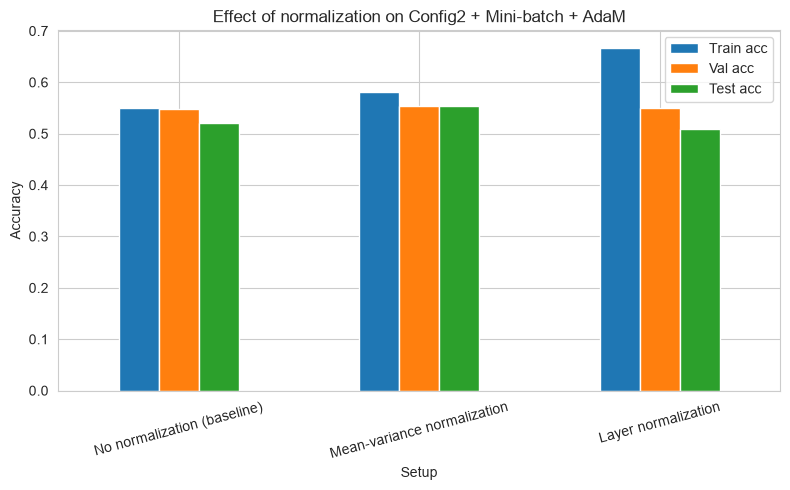
\includegraphics[width=0.44\textwidth]{normalization_comparison.png}
\end{center}

\textbf{Conclusion.} Mean-variance normalization gives the best final test result,
$55.4\%$. Layer normalization shows the largest train-test gap.

\end{document}
